\chapter{Overall Deployment}
This section describes how the previous sections, and the software components developed in each, come together to produce the final product.
\\\\
Diagram in figure \ref{fig:overall-deployment} shows the overall deployment of the software components built in this project. There are three main types of components in the diagram: 
\begin{itemize}
    \item \textbf{Active Components:} These software components are actively running as part of the final deployment of this project
    \item \textbf{One-Time Components:} These software components were manually ran and used to build the foundations of the project, but do not need to be running for the deployed product. However, they are not completely redundant now. They will be required in the future, such as for adding new Bitcoin data, performing further clustering, fetching new price data etc.
    \item \textbf{External APIs:} These components were not developed as part of this project, but serve as a datasource for the data used in this project. 
\end{itemize}
\begin{figure}[h!]
  \centering
  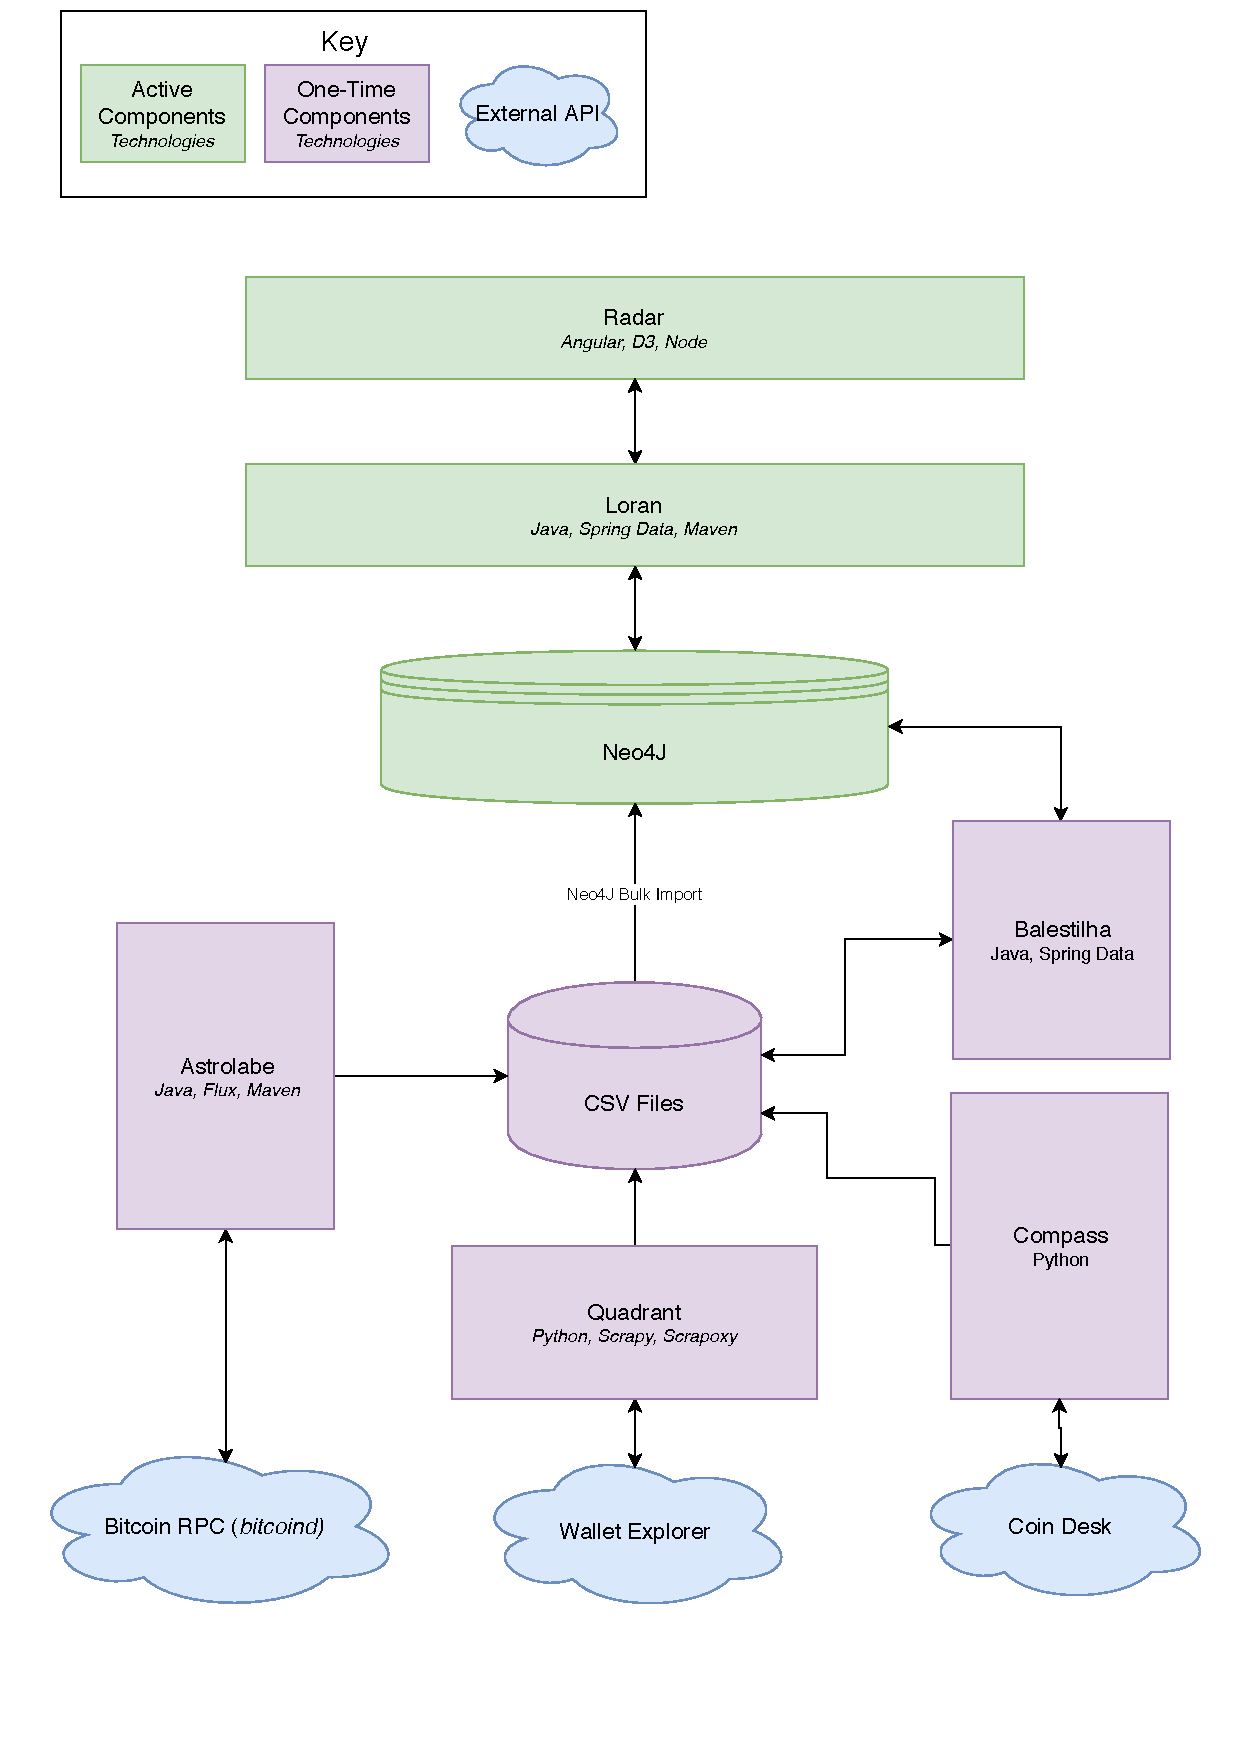
\includegraphics[width = 15cm]{./figures/overalldeployment}\\[0.5cm] 
  \caption{Overall Deployment Diagram.}
  \label{fig:overall-deployment}
\end{figure}

All components are hosted on a VM on \textit{Satoshi} [see \ref{satoshi-specs}].

\section{Developing on Satoshi}
The \textit{Satoshi} machine (and VM) is only accessible from within the Imperial College network; yet for most of this project, we worked from outside of the network. This was facilitated using multi-hop SSH tunnel and a SOCKS proxy within the web browser; all browser requests on our local machine will then be forwarded using the SOCKS proxy through port 9999, then through a SSH tunnel to the Department of Computing's public facing shell server then through another tunnel (now inside the college network) to the VM on \textit{Satoshi}. This setup can be seen in figure \ref{fig:socksproxy-setup}.
\\\\
The commands used to set up this request routing were:
\begin{itemize}
    \item On localhost: \texttt{ssh -l {login} -L  9999:localhost:9996  shell1.doc.ic.ac.uk}
    \item On DoC shell server: \texttt{ssh -l {login} -D 9996 satoshi.doc.ic.ac.uk -p 2222}
\end{itemize}
The end result was a development environment where we could navigate to localhost:8080 and localhost:7474 (for accessing \textit{Radar} and the Neo4J UI respectively) in the browser on our local machine and for all requests to be routed to the VM on Satoshi. 

\begin{figure}[h!]
  \centering
  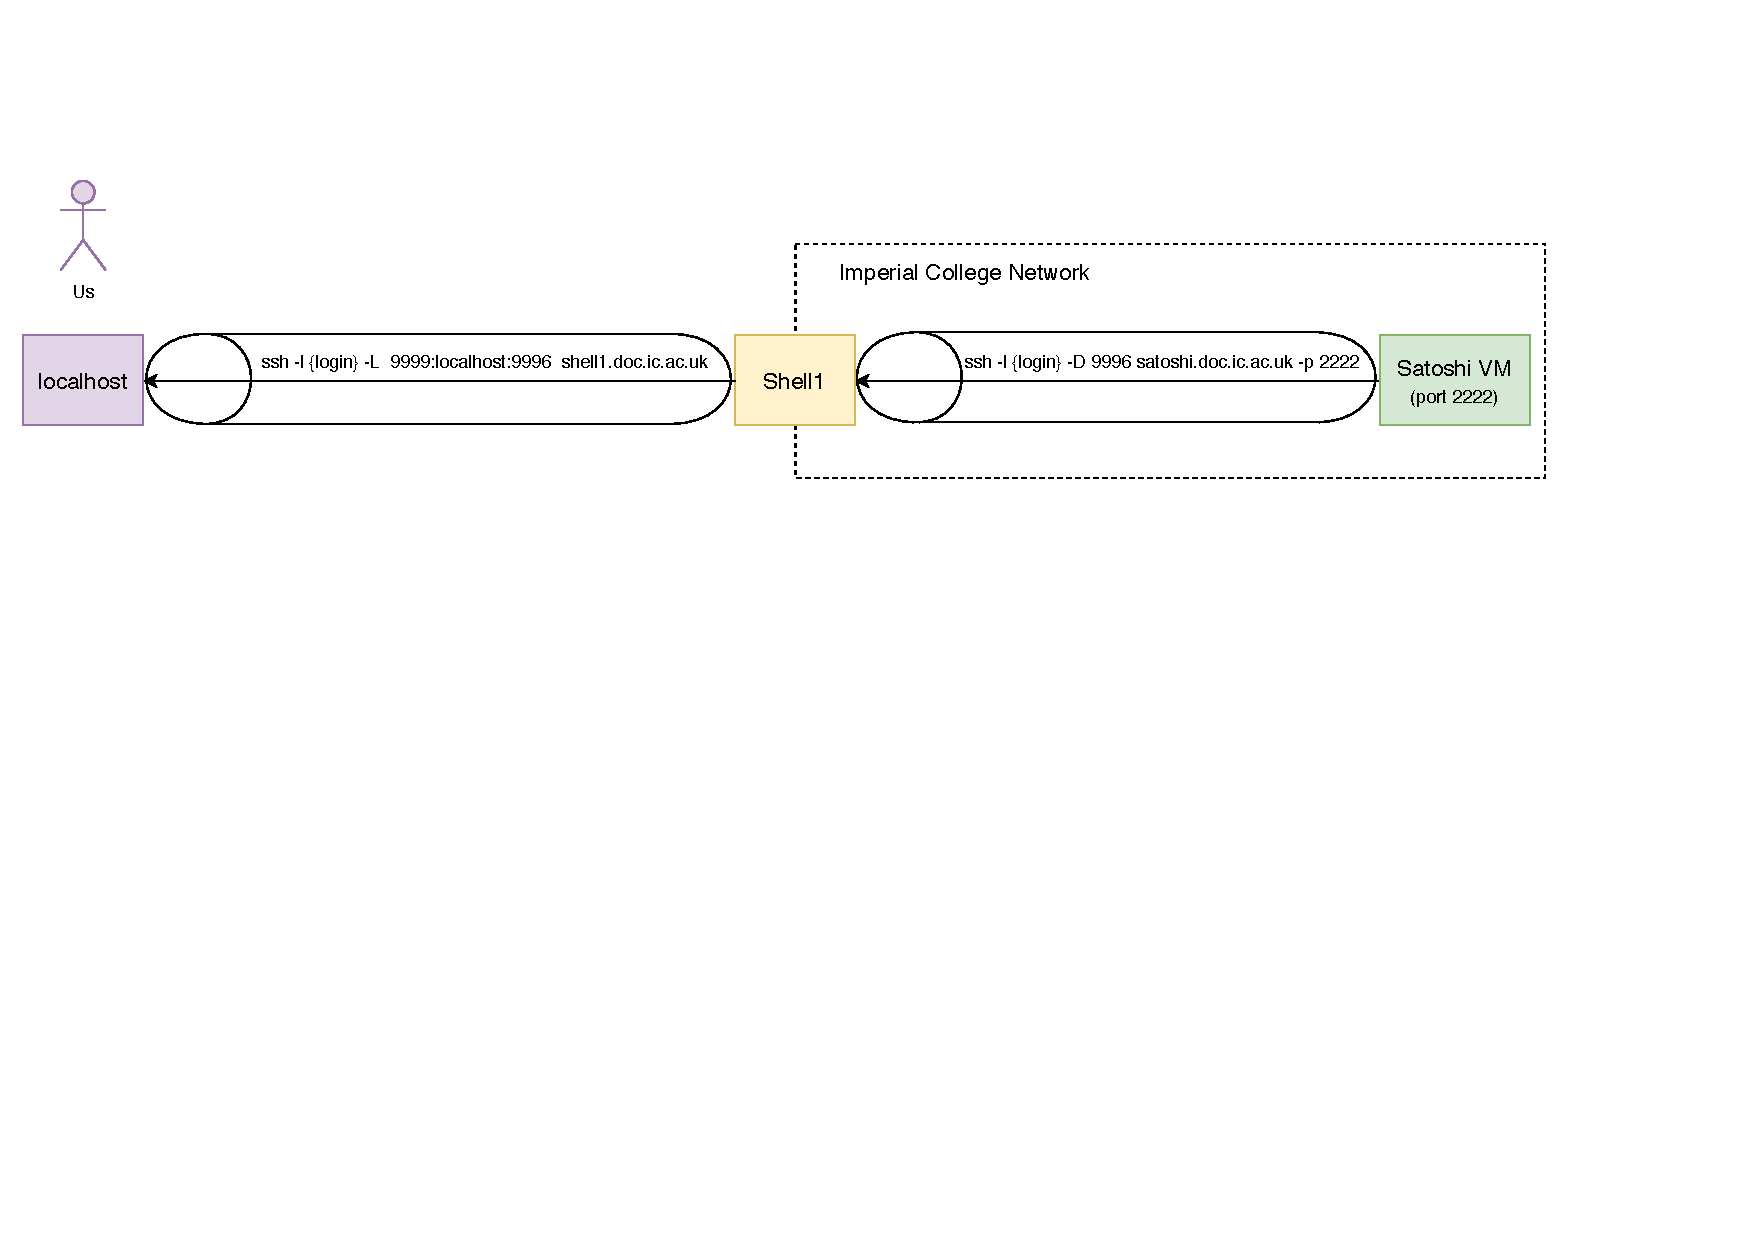
\includegraphics[width = 15cm]{./figures/socksproxyforwarding.pdf}\\[0.5cm] 
  \caption{Proxy setup for development on Satoshi from outside the Imperial network }
  \label{fig:socksproxy-setup}
\end{figure}
